% !TeX program = xelatex
\documentclass[a4paper]{article}

\input{style/ch_xelatex.tex}
\input{style/scala.tex}

%代码段设置
\lstset{numbers=left,
	basicstyle=\tiny,
	numberstyle=\tiny,
	keywordstyle=\color{blue!70},
	commentstyle=\color{red!50!green!50!blue!50},
	frame=single, rulesepcolor=\color{red!20!green!20!blue!20},
	escapeinside=``
}

\graphicspath{ {images/} }
\usepackage{ctex}
\usepackage{graphicx}
\usepackage{color,framed}%文本框
\usepackage{listings}
\usepackage{caption}
\usepackage{amssymb}
\usepackage{enumerate}
\usepackage{xcolor}
\usepackage{bm} 
\usepackage{lastpage}%获得总页数
\usepackage{fancyhdr}
\usepackage{tabularx}  
\usepackage{geometry}
\usepackage{minted}
\usepackage{graphics}
\usepackage{subfigure}
\usepackage{float}
\usepackage{pdfpages}
\usepackage{pgfplots}
\pgfplotsset{width=10cm,compat=1.9}
\usepackage{multirow}
\usepackage{footnote}
\usepackage{booktabs}

%------------------------代码-------------------
\usepackage{xcolor} 
\usepackage{listings} 
\lstset{ 
	language=Verilog, % 设置默认语言为Verilog
	breaklines,%自动换行
	basicstyle=\small\ttfamily, % 使用等宽字体
	escapeinside=``,
	keywordstyle=\color{ blue!70} \bfseries,
	commentstyle=\color{red!50!green!50!blue!50},% 
	stringstyle=\ttfamily,% 
	extendedchars=false,% 
	linewidth=\textwidth,% 
	numbers=left,% 
	numberstyle=\tiny \color{blue!50},% 
	frame=trbl,% 
	rulesepcolor= \color{ red!20!green!20!blue!20} 
}

%-------------------------页面边距--------------
\geometry{a4paper,left=2.3cm,right=2.3cm,top=2.7cm,bottom=2.7cm}
%-------------------------页眉页脚--------------
\usepackage{fancyhdr}
\pagestyle{fancy}
\lhead{\kaishu \leftmark}
% \chead{}
\rhead{\kaishu 计算机体系结构实验报告}%加粗\bfseries 
\lfoot{}
\cfoot{\thepage}
\rfoot{}
\renewcommand{\headrulewidth}{0.1pt}  
\renewcommand{\footrulewidth}{0pt}%去掉横线
\newcommand{\HRule}{\rule{\linewidth}{0.5mm}}%标题横线
\newcommand{\HRulegrossa}{\rule{\linewidth}{1.2mm}}
\setlength{\textfloatsep}{10mm}%设置图片的前后间距
%--------------------文档内容--------------------

\begin{document}
	\renewcommand{\contentsname}{目\ 录}
	\renewcommand{\appendixname}{附录}
	\renewcommand{\appendixpagename}{附录}
	\renewcommand{\refname}{参考文献} 
	\renewcommand{\figurename}{图}
	\renewcommand{\tablename}{表}
	\renewcommand{\today}{\number\year 年 \number\month 月 \number\day 日}
	
	%-------------------------封面----------------
	\begin{titlepage}
		\begin{center}
			
\includegraphics[width=0.8\textwidth]{NKU.png}\\[1cm]
			\vspace{20mm}
			\textbf{\huge\textbf{\kaishu{计算机学院}}}\\[0.5cm]
			\textbf{\huge{\kaishu{计算机体系结构实验报告}}}\\[2.3cm]
			\textbf{\Huge\textbf{\kaishu{旁路前递}}}
			
			\vspace{\fill}
			
			% \textbf{\Large \textbf{计算机体系结构实验报告}}\\[0.8cm]
			% \HRule \\[0.9cm]
			% \HRule \\[2.0cm]
			\centering
			\textsc{\LARGE \kaishu{姓名\ :\ 王一诺}}\\[0.5cm]
			\textsc{\LARGE \kaishu{学号\ :\ 2312331}}\\[0.5cm]
			\textsc{\LARGE \kaishu{专业\ :\ 计算机科学与技术}}\\[0.5cm]
			\textsc{\LARGE \kaishu{指导老师\ :\ 董前琨}}\\[0.5cm]
			
			\vfill
			{\Large \today}
		\end{center}
	\end{titlepage}
	
	\renewcommand {\thefigure}{\thesection{}.\arabic{figure}}%图片按章标号
	\renewcommand{\figurename}{图}
	\renewcommand{\contentsname}{目录}  
	\cfoot{\thepage\ of \pageref{LastPage}}%当前页 of 总页数
	
	
	% 生成目录
	\clearpage
	\tableofcontents
	\newpage
	\setcounter{figure}{0} % 每章开始前重置图片计数器
	
	
	\section{实验要求}
	请在第一次实验的五级流水线CPU的基础上，根据《CPU设计实战》这本书上第四章后面的内容，验证现有CPU的指令相关和流水线冲突问题，以添加旁路的方式和前递技术，让CPU规避这样的问题。注意：
	\begin{enumerate}
		\item 实验报告中简要画一下旁路设计的示意图，有对应的介绍
		\item 实验结果要进行详细分析，原始情况下指令是如何执行的，增加了旁路和前递之后是如何执行的
	\end{enumerate}
	
	\section{指令相关与流水线冲突}
	根据实验指导书，关于指令相关与流水线冲突的原理性阐述可以总结为以下几点：
	\begin{enumerate}
		\item 单发射静态流水线上只需要解决围绕寄存器的写后读数据村相关所引发的流水线冲突,围绕寄存器的写后写和读后写数据相关不会引发流水线冲突,围绕内存的所有类型的数据相关也不会引发流水线冲突。
		\item 对于单发射静态流水的MIPS CPU,如果取指和译码阶段没均只设计为一级流水线,那么只需要在译码阶段进行转移指令的处理,就能够在完全不阻塞(清空)流水线的情况下解决控制相关引发的流水线冲突。
		\item 单发射静态流水线上的结构相关所引发的流水线冲突的处理可以简化为:后一级流水线的指令无法运行,则前一级流水线的指令也无法运行。
	\end{enumerate}
	
	针对第2点,当前的流水线CPU设计已经将所有转移指令的处理都放在译码阶段了，所以控制相关的流水线冲突已经得到解决；
	
	针对第3点,当前的流水线CPU设计中所采用的逐级互锁控制机制能够确保任何一级无法前行时,它前面的所有流水级都可以及时停止,同时不丢失数据,所以结构相关引发的流水线冲突也已经得到解决。
	
	接下来主要关注解决写后读数据相关所引发的流水线冲突。
	
	\section{阻塞译码级}
	产生由寄存器写后读数据相关所引发的流水线冲突的场景是:产生结果的指令("写者")尚未将结果写回到通用寄存器堆中,而需要这个结果的指令("读者")已经在译码阶段了,此刻它从通用寄存器堆中读出的数值是旧值而非新值。
	
	如何避免产生这种错误呢?观察当前的代码实现，其实已经采用了阻塞的方式进行了简单解决，直观点描述思路就是:让需要结果的指令在详码流水级一直等待,直到产生结果的指令将结果写入到通用寄存器堆,才可以进入到下一级的执行流水级中。
	
	这套设计思路中的关键点在于控制译码流水级指令前进还是阻塞的条件如何生成,其核心是判断处于流水线不同阶段的指令是否存在会引发冲突的"写后读"相关关系。结合我们设计的五级流水线CPU的结构,这个判断可以具体描述为:处于译码流水级的指令具有来自非0号寄存器的源操作数,那么如果这些源操作数中任何一个的寄存器号与当前时刻处于执行级、访存级或写回级的指令的目的操作数的寄存器号(非0号)相同,则表明处于译码级的指令与执行级、访存级或写回级的指令存在会引发冲突的为"写后读"相关关系。
	
	\begin{lstlisting}[caption={decode阶段比对源操作数并阻塞}]
		// =========================================================================
		// 数据冒险检测：与后级目的寄存器冲突时阻塞译码级。
		// =========================================================================
		wire rs_wait;
		wire rt_wait;
		assign rs_wait = ~inst_no_rs & (rs!=5'd0)
		& ( (rs==EXE_wdest) | (rs==MEM_wdest) | (rs==WB_wdest) );
		assign rt_wait = ~inst_no_rt & (rt!=5'd0)
		& ( (rt==EXE_wdest) | (rt==MEM_wdest) | (rt==WB_wdest) );
		assign ID_over = ID_valid & ~rs_wait & ~rt_wait & (~inst_jbr | IF_over);
	\end{lstlisting}
	
	可以注意到，当前的代码在阻塞的判定时还考虑了跳转指令，BEQ/BNE/JR/JALR 等转移类指令未被豁免在inst\_no\_rs与inst\_no\_rt中。这其实是对“转移计算未完成”的分析。
	
	在"写后读"相关中存在一种情况--Load-to-Branch,即第i条指令是Load,第i+1条指令是转移(跳转或分支)指令,转移指令至少有一个源寄存器与Load指令的目的寄存器相同,也就是Branch与Load存在"写后读相关"。在这种情况下,当转移指令在译码级时,Load指令在执行级无法获得Load结果,因而转移指令无法计算正确的跳转方向或跳转目标,称为"转移计算未完成"。因此这里译码级会在检测到前序 Load 尚未写回时阻塞后续转移/分支指令。
	
	\section{旁路前递}
	旁路前递（forwarding），直观来看就是给流水线多铺几条“捷径”，连着执行级、访存级、写回级的运算结果与信号。原代码基础工程只依赖寄存器堆同步写回，任何一条算术指令都要等到写回级落地之后译码级才能看到寄存器的新值，当发生数据相关情况时只能"阻塞"译码阶段等待前条指令的完成，这无疑带来了不小的时间开销。为了解除这一瓶颈，我们让译码级可以直接引用执行级、访存级甚至写回级即将写回的结果，并在每个阶段配套一位“结果已就绪”的标志位。这就是“旁路前递”。
	\subsection{前递路径设计}
	实验书其实给出了两种旁路的设计思路：
	\begin{enumerate}
		\item "流水级组合逻辑结果前递到译码级寄存器读出"
		\item "流水级缓存保存的前一级结果前递到执行级ALU输入"
	\end{enumerate}
	
	简单分析一下这两种方案。为了尽可能多地通过前递来消除指令阻塞带来的性能损失,可以发现无论是哪套方案,都需要将前递路径的终点放在译码级寄存器堆读出结果生成逻辑处。相比之下倾向于方案一,这样所有的前递路径终点一致,使使得由前递结果生成正确的寄存器源操作数的逻辑可以在一个地方集中处理。此外，考虑到所有转移指令的处理都被放在译码级，BEQ、BNE、JR指令都有寄存器源操作数，还是前递路径的终点位于译码级更加方便。综上，采取第一种方案设计来实现旁路前递。
	
	简易设计图如下：
	\begin{figure}[H]
		\centering
		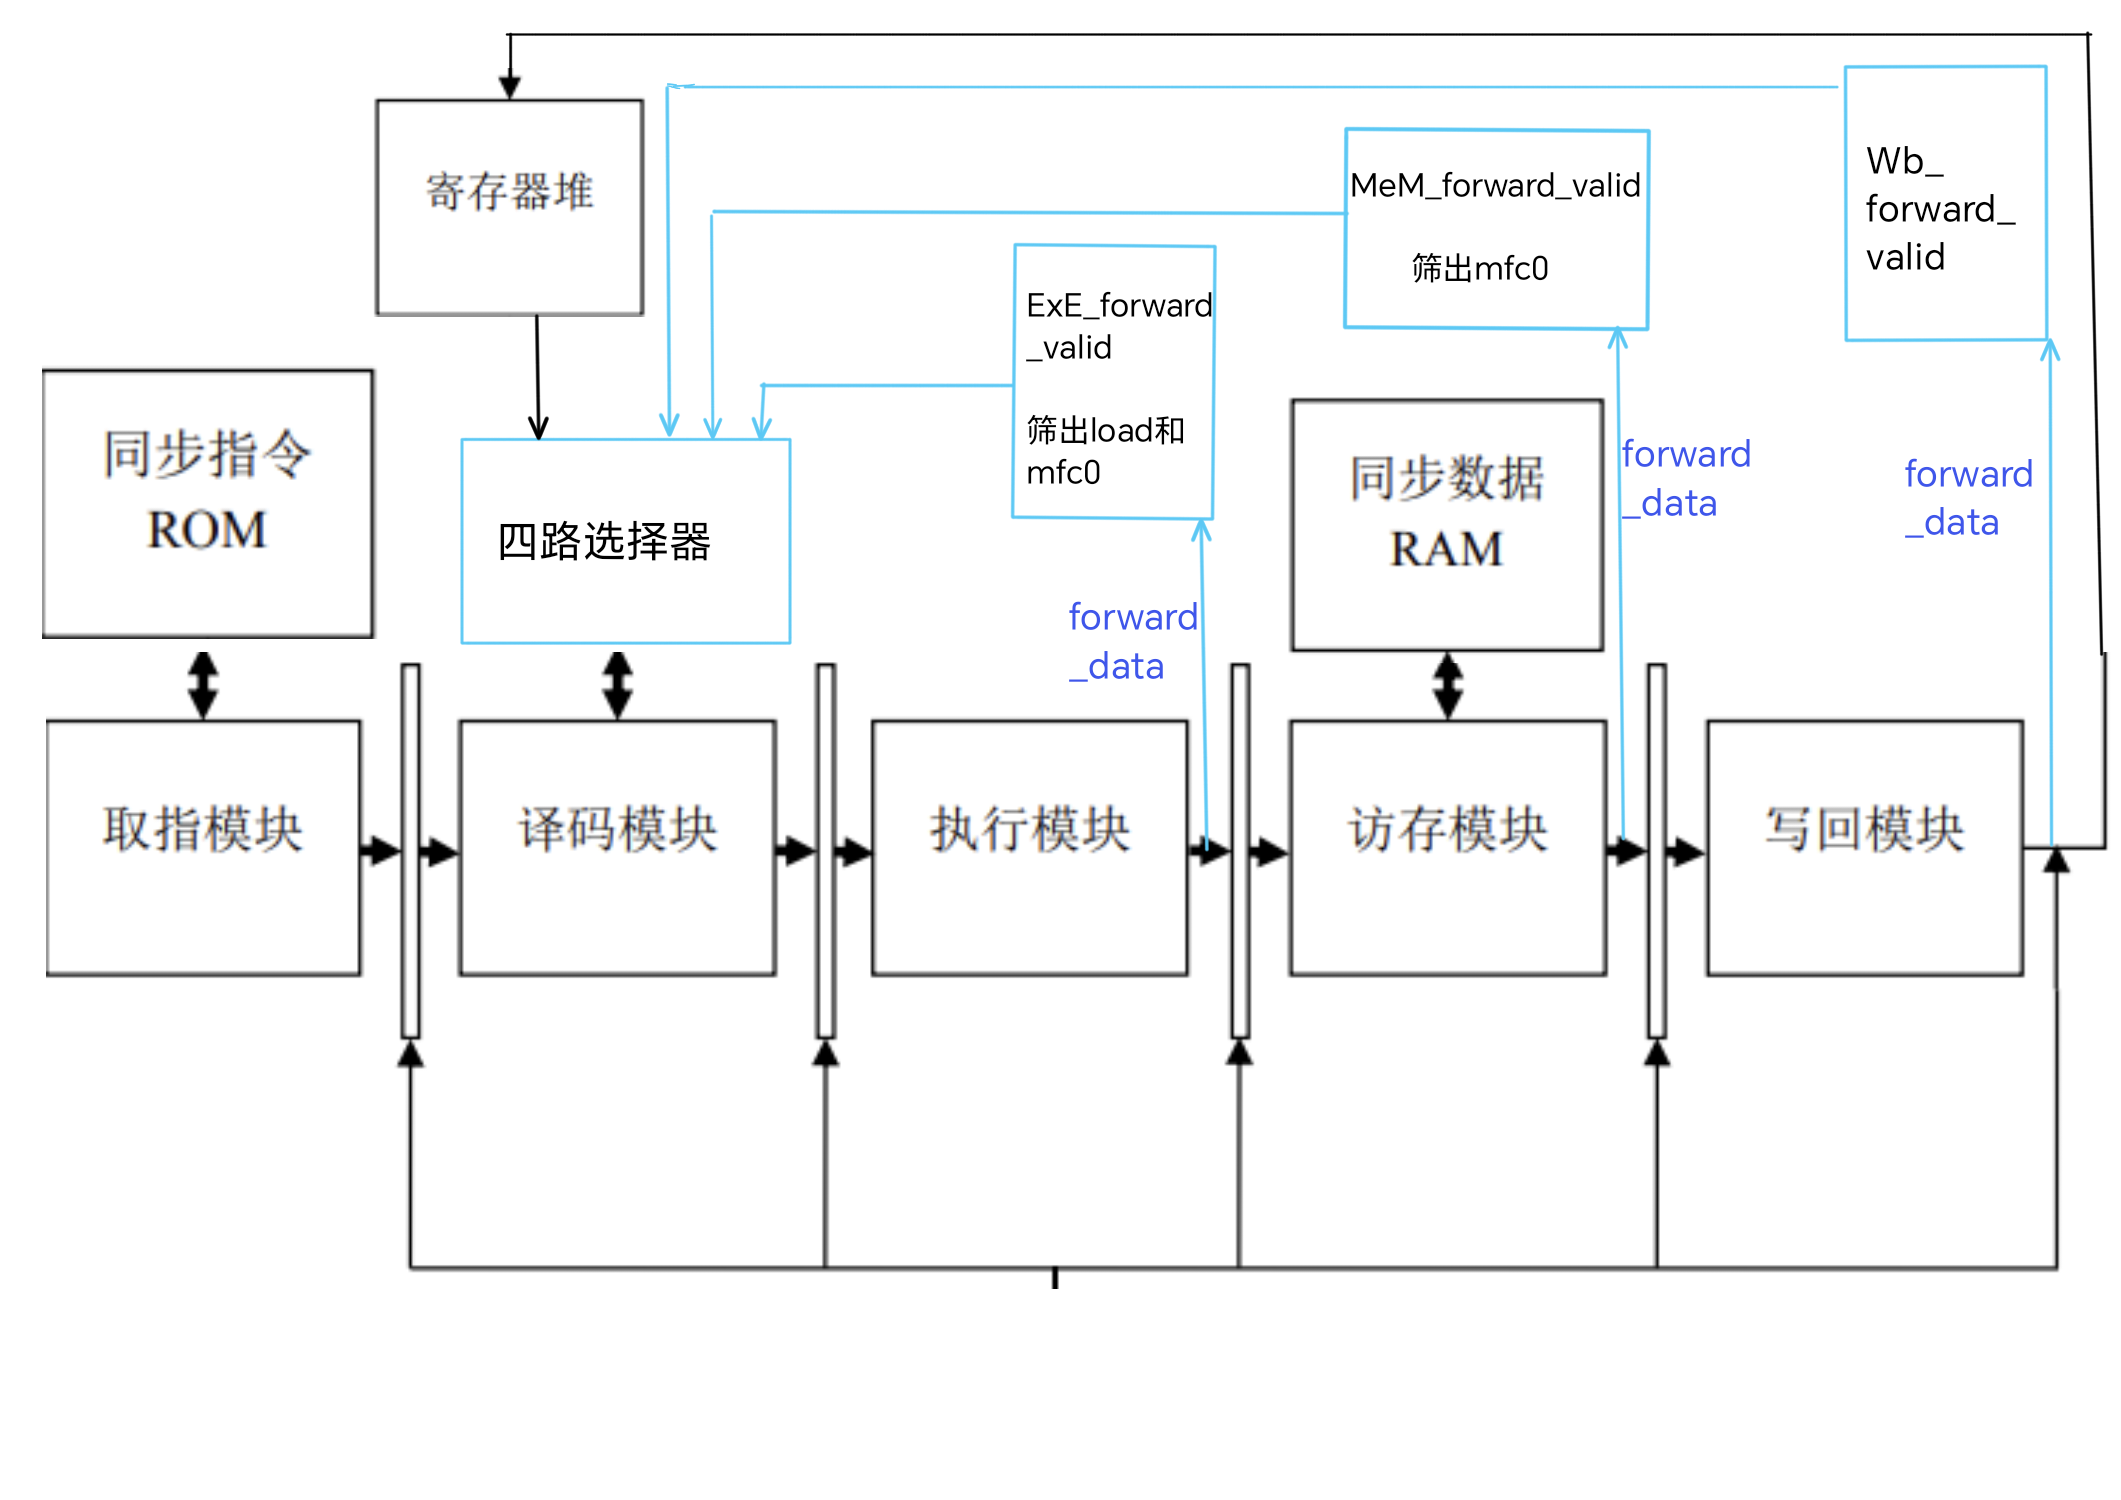
\includegraphics[width=\textwidth]{sheji.png}
		\caption{旁路方案设计图}
		\label{fig:sheji}
	\end{figure}
	
	那么，接下来我们在译码级之后的每一个流水级都添加一条重点在译码级的前递路径并设计好前递数据和标志位来实现该方案。
	
	\paragraph{执行级} exe.v
	
	执行级的改动集中在输出端口和有效标志的判断。新增了 `EXE\_forward\_data` 与 `EXE\_forward\_valid` 两个输出，其中 `EXE\_forward\_data` 直接复用 `exe\_result`，而有效性由以下语句控制：
	\begin{lstlisting}[caption={exe.v}]
		assign EXE_forward_valid = EXE_valid & rf_wen
									& ~inst_load
									& ~mfc0
									& (~multiply | mult_end);
	\end{lstlisting}
	
	`EXE\_valid \& rf\_wen` 说明当前拍携带的指令会写通用寄存器；`~inst\_load` 把同步 RAM 的结果排除在外，这里其实是对load-use情况的关照考虑，load指令还是要阻塞到mem阶段，不能在exe级前递；`~mfc0` 对应 CP0 读取的特殊时序——`mfc0` 在执行级只得到占位值，真正的读数要到写回级才出现，因此在执行级不应该前递，这其实类似对load-use的处理，但是第一次改写代码时并未考虑该情况而导致了exception退回失败，后文将会详细说明该问题；`(~multiply | mult\_end)` 则确保乘法器在 `mult\_end` 拉高之前不会提前对外宣称结果可用。`inst\_load` 来自对 `mem\_control` 的拆包，`mfc0` 与 `multiply` 等信号均由译码级一路传递过来，所以执行级只需组合现成信号即可。
	
	\paragraph{访存级} mem.v
	
	访存级增加了 `MEM\_forward\_data` 与 `MEM\_forward\_valid`。旁路数据统一取 `mem\_result`，它在 load 时选用 RAM 的返回值，其余指令沿用执行级的运算结果。有效标志为：
	\begin{lstlisting}[caption={mem.v}]
		assign MEM_forward_valid = MEM_over & rf_wen & ~mfc0;
	\end{lstlisting}
	
	其中 `MEM\_over` 意味着同步 RAM 的读数据已经被锁存，`rf\_wen` 依旧限制在写通用寄存器的指令范围内，`~mfc0` 避免 CP0 读结果再次被提前获取。因为 load 指令原本就通过 `MEM\_valid\_r` 额外等待一拍，旁路逻辑只需判断 `MEM\_over` 即可知道结果是否稳定。
	
	\paragraph{写回级} wb.v
	写回级本身不需要新增或删改代码，它天生就满足旁路所需的“数据 + 有效标志”接口：wb.v 把 rf\_wen 定义成 wen \& WB\_over，只有真正完成写回时才拉高；把最终写回数据整理成 rf\_wdata，还有 WB\_wdest 供外部做相关判断。直接把写回级现成的 rf\_wdata、rf\_wen 作为 WB 级的旁路数据和有效标志直接接回译码级即可。
	
	\paragraph{顶层} pipeline\_cpu.v
	
	顶层只负责组织连线：声明 `EXE\_forward\_*`、`MEM\_forward\_*`，在实例化 `decode`、`exe`、`mem` 时补齐端口，并把写回级的 `rf\_wdata`、`rf\_wen` 直接送到译码级作为 WB 旁路数据与有效标志。旁路不会绕过寄存器堆写口，写回仍按原计划写入寄存器堆，用于后续完全无关的指令读取。
	
	\subsection{前递结果的多路选择}
	前递路径就这样建好了，但是译码级寄存器读结果该读取哪个呢？是读取前递回来的还是当前的，又是读取哪个流水级前递回来的结果呢？这就需要设计译码级寄存器读结果的多路选择逻辑。选择哪个前递结果,不仅要看源操作数的寄存器号与前递来的结果的寄存器号是否一致,还要考虑不同流水级之间的优先级关系。
	
	首先，什么时候需要采用前递结果也就是如何判定数据相关问题呢？显而易见，当前指令读取的寄存器号与前递的寄存器号相同时就说明发生了数据相关，很容易能写出以下代码：
	\begin{lstlisting}[caption={decode.v}]
		wire        rs_need;
		wire        rt_need;
		wire        rs_match_exe;
		wire        rs_match_mem;
		wire        rs_match_wb;
		wire        rt_match_exe;
		wire        rt_match_mem;
		wire        rt_match_wb;
		
		assign rs_need = ~inst_no_rs & (rs != 5'd0);
		assign rt_need = ~inst_no_rt & (rt != 5'd0);
		
		assign rs_match_exe = rs_need & (rs == EXE_wdest);
		assign rs_match_mem = rs_need & (rs == MEM_wdest);
		assign rs_match_wb  = rs_need & (rs == WB_wdest);
		assign rt_match_exe = rt_need & (rt == EXE_wdest);
		assign rt_match_mem = rt_need & (rt == MEM_wdest);
		assign rt_match_wb  = rt_need & (rt == WB_wdest);
	\end{lstlisting}
	这就给我们的多路选择提供了控制信号。
	
	接下来解决流水级优先级的问题。其实很容易理解：当前指令用到的数据被指前几条指令动用了，那么我们肯定需要使用最新的数据，也就是与当前指令有数据相关问题的指令中距离当前指令最近的那个，而距离当前指令越近，其所在的流水级也就应该离译码级（当前指令所在的流水级）越近。所以我们得到：应该按照EXE → MEM → WB 的优先级去挑选数据；当然，没有数据相关时就采用当前读取的数据。此外，不要忘记能偶使用前递结果的条件——forward\_valid，这些在前面的路径设计部分已经说明，用来设定正确的前递时机。相关代码如下：
	\begin{lstlisting}[caption={decode.v}]
	    assign rs_data = rs_match_exe && EXE_forward_valid ? EXE_forward_data :
						 rs_match_mem && MEM_forward_valid ? MEM_forward_data :
						 rs_match_wb  && WB_forward_valid  ? WB_forward_data  :
					                                         rs_value;
	
		assign rt_data = rt_match_exe && EXE_forward_valid ? EXE_forward_data :
						 rt_match_mem && MEM_forward_valid ? MEM_forward_data :
						 rt_match_wb  && WB_forward_valid  ? WB_forward_data  :
														     rt_value;   
	\end{lstlisting}
	
	所有原先依赖 rs\_value/rt\_value 的逻辑——包括跳转目标、比较结果、ALU 操作数以及 store 写数据——都换成了 rs\_data/rt\_data。这样就完成了对前递结果的多路选择的设计。
	
	\subsection{流水线控制信号调整}
	最后一步就是要对阻塞逻辑进行调整，能取前递结果时就取消阻塞，这也是旁路前递相比原有阻塞方案能节省用时的原因。
	
	原有方案是按照最严格的方式阻塞，采取旁路前递后，就可以根据前面写好的多路选择逻辑取用正确的前递结果，阻塞判定就可以放宽：没有一个match时或者forward\_valid都为0（表示对应流水级还没有产生正确结果，还未发生前递）时才阻塞；一旦match信号和forward\_valid有效位拉高，则立即取消阻塞。相关代码如下：
	\begin{lstlisting}[caption={decode.v}]
		wire rs_wait;
		wire rt_wait;
		assign rs_wait = rs_match_exe ? ~EXE_forward_valid :
						 rs_match_mem ? ~MEM_forward_valid :
						 rs_match_wb  ? ~WB_forward_valid  :
										1'b0;
	
		assign rt_wait = rt_match_exe ? ~EXE_forward_valid :
						 rt_match_mem ? ~MEM_forward_valid :
						 rt_match_wb  ? ~WB_forward_valid  :
										1'b0;
										
		assign ID_over = ID_valid & ~rs_wait & ~rt_wait & (~inst_jbr | IF_over);
	\end{lstlisting}
	
	至此就完成了完整的旁路前递设计。
	
	\section{仿真结果与分析}
	通过仿真，可以很明显地看到指令所用周期的缩短，接下来以前几条指令为例简单分析一下。
	
	首先分析一下前几条指令是什么，有哪些会产生数据依赖的情况：
	\begin{lstlisting}[caption={analysis}]
		  PC     Hex           汇编         依赖      说明
	I1	0x34   24010001   addiu  r1,r0,1    -        产生 r1
	I2	0x38   00011100   sll    r2,r1,4    r1←I1    立即依赖
	I3	0x3C   00411821   addu   r3,r2,r1   r2,r1    双重依赖
	I4	0x40   00022082   srl    r4,r2,2    r2       连续依赖
	I5	0x44   28990005   slti   r25,r4,5   r4       
	I6	0x48   0721000E   bgez   r25,+14    r25      分支判断
	\end{lstlisting}
	
	运行原有阻塞方案，观察仿真结果：
	\begin{figure}[H]
		\centering
		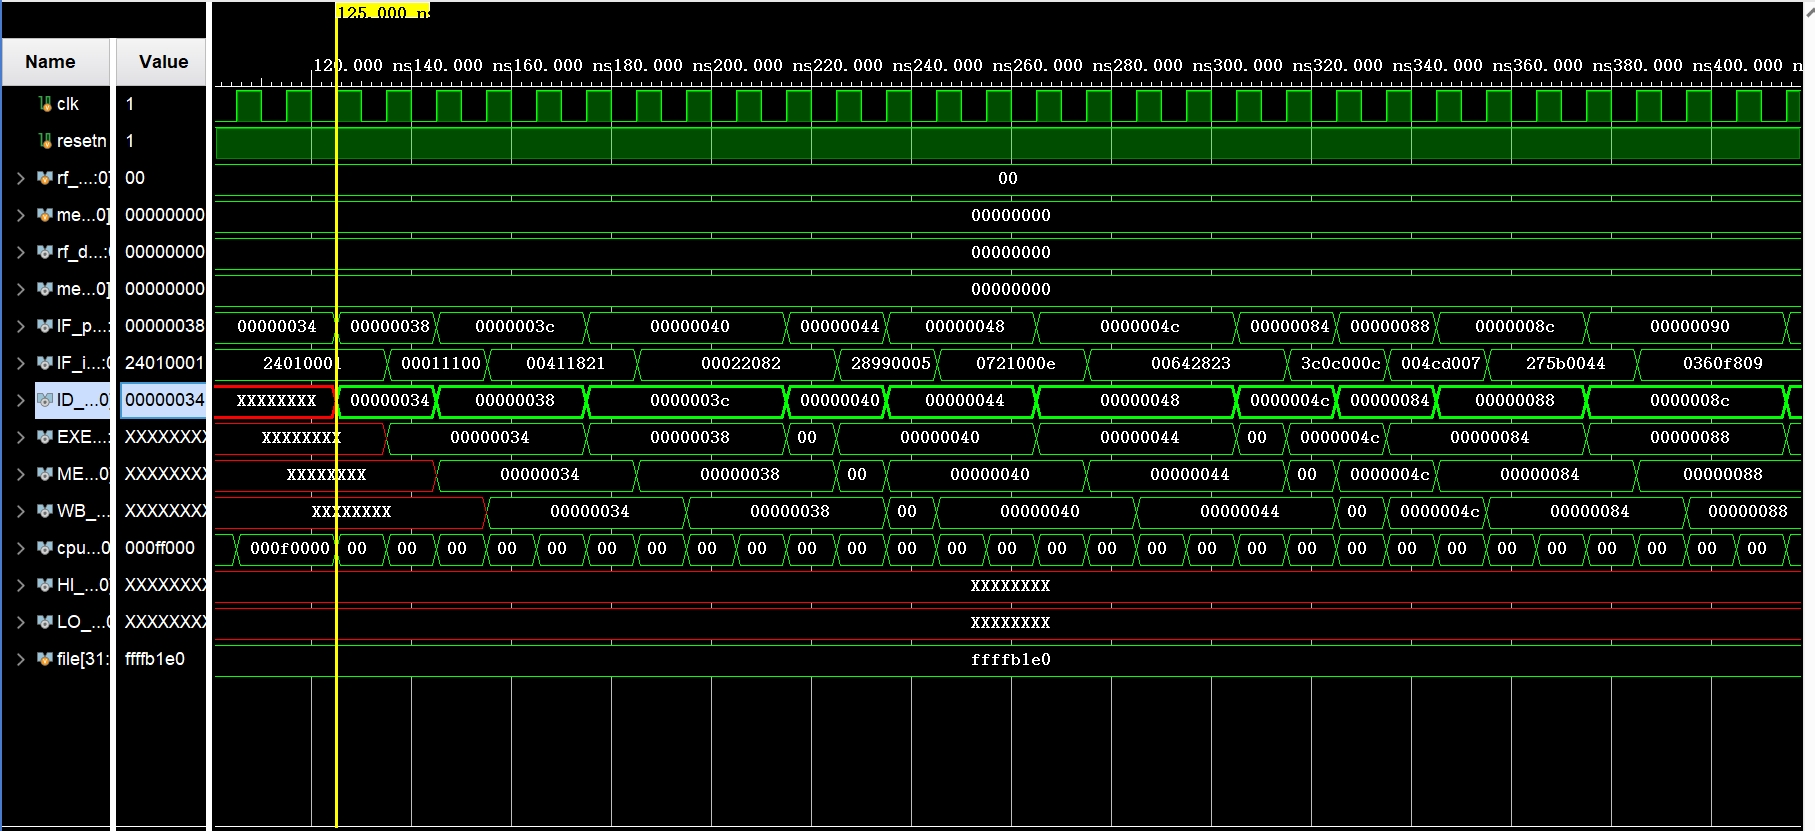
\includegraphics[width=\textwidth]{zuse.png}
		\caption{阻塞方案仿真}
		\label{fig:zuse}
	\end{figure}
	
	运行旁路前递方案，观察仿真结果：
	\begin{figure}[H]
		\centering
		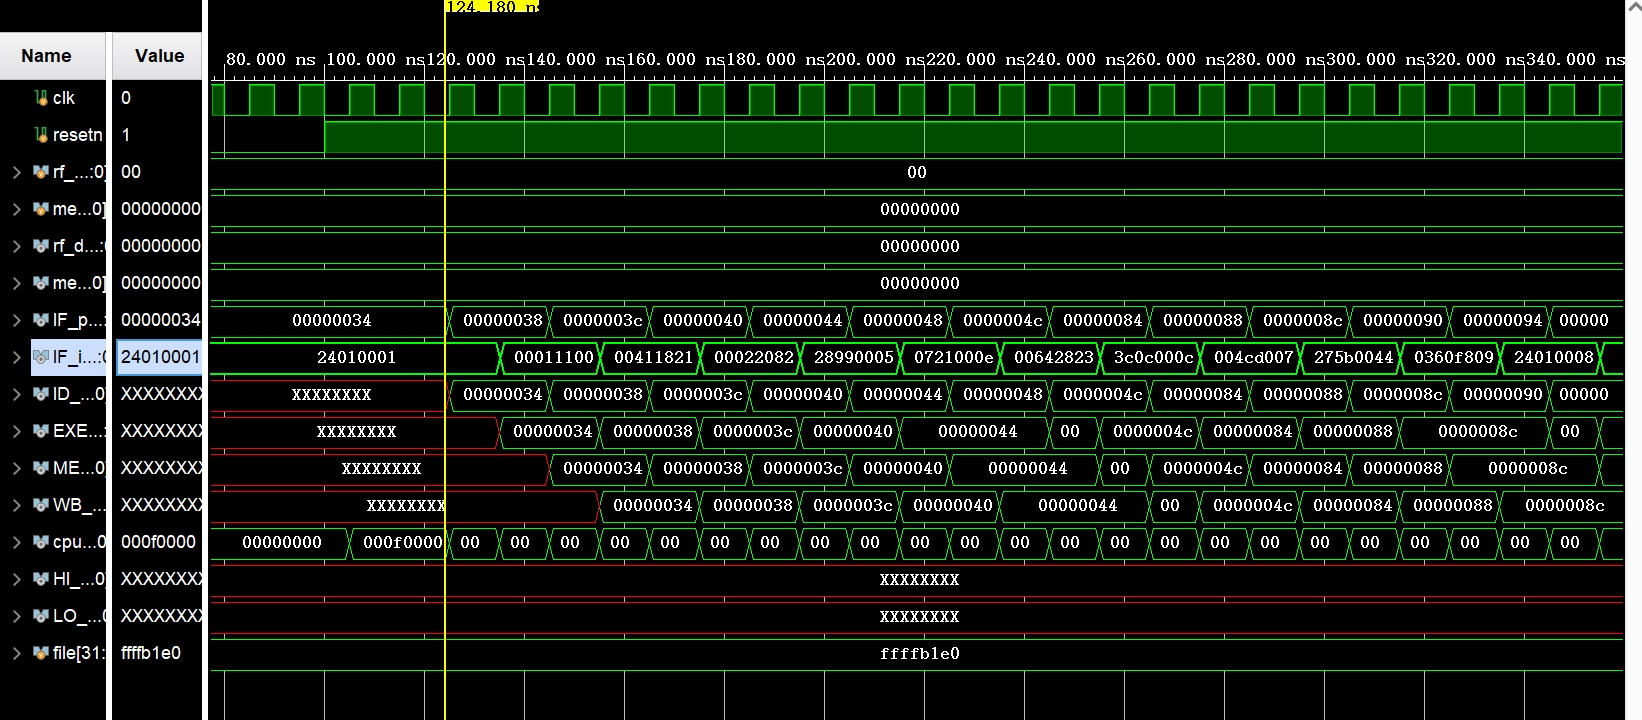
\includegraphics[width=\textwidth]{panglu.png}
		\caption{旁路方案仿真}
		\label{fig:panglu}
	\end{figure}
	
	对比分析一下在这几条指令的运行上两个方案的差异：
	\paragraph{addi \$1,\$0,1} (PC=0x00000034)
	
	旁路方案：各级 3/2/2/2/2拍。
	
	IF 复位后按照 IF\_allow\_in = IF\_over \& ID\_allow\_in 正常推进；ID 没有数据相关，rs\_wait/rt\_wait 直接为 0；EXE~WB 每级只用两个周期完成，未出现停顿。
	
	严格阻塞：3/2/4/4/4拍。
	
	下一条 sll 需要 \$1，decode.v 检测到 rs==EXE\_wdest 令 rs\_wait=1，从而 ID\_over=0；原方案的设计机制要求 EXE\_over \& MEM\_allow\_in 才能前推，因此 EXE/MEM/WB 被迫保持该指令整整 4 拍，直到写回结束才释放。
	
	\paragraph{sll \$2,\$1,4}(PC=0x00000038)
	
	旁路方案：2/2/2/2/2拍。
	
	decode.v 将 EXE产生的 \$1 直接前递给 rs\_data，rs\_wait 立即清零，所以 ID 只停两拍，后端保持满速。
	
	严格阻塞：2/3/4/4/4拍。
	
	由于没有前递，decode.v 仍判定 \$1 在 EXE/MEM/WB 中，ID连续三拍保持等待；源代码的链式阻塞让 EXE~WB 再次各延长到 4 拍。
	
	\paragraph{addu \$3,\$2,\$1} (PC=0x0000003C)
	
	旁路方案：2/2/2/2/2拍。
	
	sll 与 addi 的结果分别从 EXE/MEM 前递，因此 ID 一次性拿到\$2/\$1；EXE\_forward\_valid 也为真，整个流水线保持顺畅。
	
	严格阻塞：3/4/1/1/1拍。
	
	此时 \$2 尚在 EXE、\$1 正在 MEM，比分别写回晚两拍，rs\_wait/rt\_wait 始终为 1，IF 也被迫等待 3 拍。待两源数真正写回后，指令才在 EXE 迅速完成并一路冲过 MEM/WB。
	
	\paragraph{srl \$4,\$2,2} (PC=0x00000040)
	
	旁路方案：2/2/2/2/2拍。
	
	sll 的结果继续通过前递口进入 ID，未触发等待；链路保持打通。
	
	严格阻塞：4/2/4/4/4拍。
	
	因为 \$2 还在前级，decode.v再次抬高 rs\_wait，IF 连续四拍取到同一 PC；直到 \$2 真正在 WB 写回后，EXE~WB 逐级释放。
	
	\paragraph{slti \$25,\$4,5} (PC=0x00000044)
	
	旁路方案：2/2/3/3/3拍。
	
	数据相关已靠前递解决，但后续分支需要本指令的比较结果才能决定走向。为保证 inst\_jbr 在 ID 看到稳定数值，decode.v要求 branch 等待 IF\_over=1，因此当分支仍在 IF/ID 决策时，链路暂时冻结 EXE/MEM/WB 一拍，让比较结果在流水尾部多保留一周期供分支采样。
	
	严格阻塞：2/3/4/4/4拍。
	
	除去与旁路方案相同的分支等待，还叠加了 \$4 未写回导致的 rs\_wait=1，使 ID 多卡一拍、EXE~WB 各再多一拍。
	
	\paragraph{bgez \$25,+0xE} (PC=0x00000048)
	
	旁路方案：2/2/1/1/1拍。
	
	slti 在 EXE 就输出比较结果，将其前递到 ID；rs\_wait 立刻拉低，branch 只在 ID 停留两拍，同时通过与 IF\_over协调完成重定向，因此 EXE 级仅需一拍做出跳转决策。
	
	严格阻塞：3/4/1/1/1拍。
	
	由于 \$25 要等 WB 写回，decode 让 rs\_wait 四拍为 1，ID 与 IF 长时间冻结；直到写回完成后分支才在 EXE 判定，并在一个拍内刷新 PC。
	
	\paragraph{结论}
	
	- 原始严格阻塞方案依赖 decode.v 的简单资源占用检查，任何 RAW 相关都会让 ID\_over 变 0，进而把停顿传递到全部后级，导致 EXE/MEM/WB 集体“抱团”多拍。
	
	- 旁路版通过多级前递和细粒度等待判定，只在确实无法前递（如负载、CP0、乘法未完成）时才阻塞，因此大部分算术逻辑指令恢复到 2 拍节奏。
	
	- 结果上，旁路方案在 255000ns 就把 PC 推进到 0x00000084，严格阻塞直到 315000ns 才到同
	样位置，验证了旁路前递显著压缩了数据相关引起的多级停顿。
	
	\section{关于mfc0}
	前面提及了mfc0的问题——在实验书写中，曾出现了在00000104进入exception00000000~00000030后没有正常回到00000108继续执行反而困在exception内的问题，如下图：
	\begin{figure}[H]
		\centering
		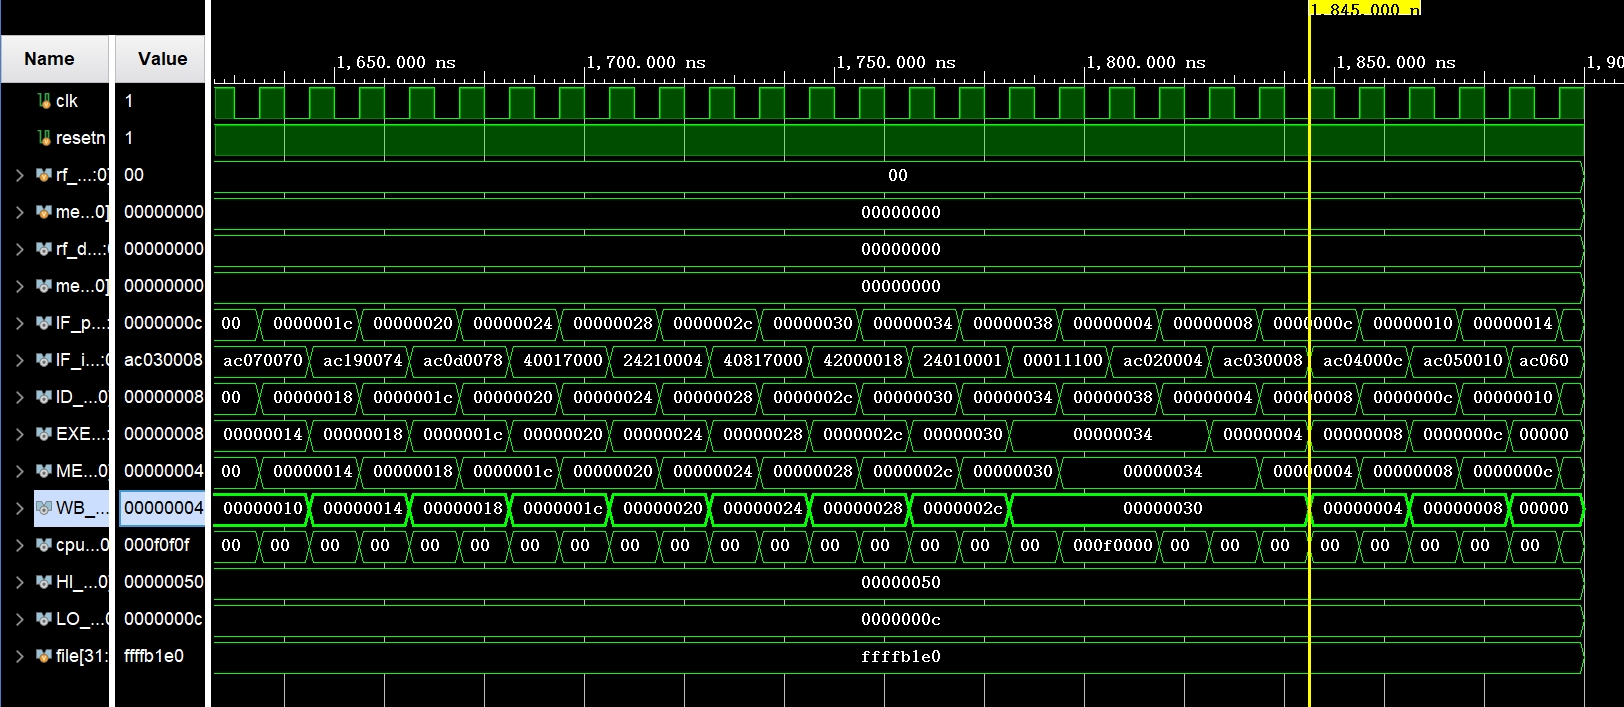
\includegraphics[width=\textwidth]{bug.png}
		\label{fig:bug}
	\end{figure}
	
	仔细检查后发现，EXE\_forward\_valid和MEM\_forward\_valid的判定逻辑中没有把mfc0剔除，此时异常处理序列 mfc0 -> addiu -> mtc0 -> eret 会把 EPC 写成 0x00000004。原因是执行级在 mfc0 时只输出占位零值，译码级立刻把这个伪结果当成有效数据，导致 addiu 之后再写回 CP0 时地址被覆盖，也就使得程序困在exception内了。
	
	解决方案也十分简单，将 ~mfc0 纳入 EXE\_forward\_valid 与 MEM\_forward\_valid 之后，译码级会乖乖等待到写回级的 rf\_wdata 真正携带 EPC，这样 eret 才能正确返回到 0x00000108。
	
	\begin{lstlisting}[caption={bugmix}]
		assign EXE_forward_valid = EXE_valid & rf_wen
										& ~inst_load
										& ~mfc0
										& (~multiply | mult_end);
										
		assign MEM_forward_valid = MEM_over & rf_wen & ~mfc0;
	\end{lstlisting}
	
	这很类似我们对"load-use"的处理。
	
	解决问题后波形如下图：
	\begin{figure}[H]
		\centering
		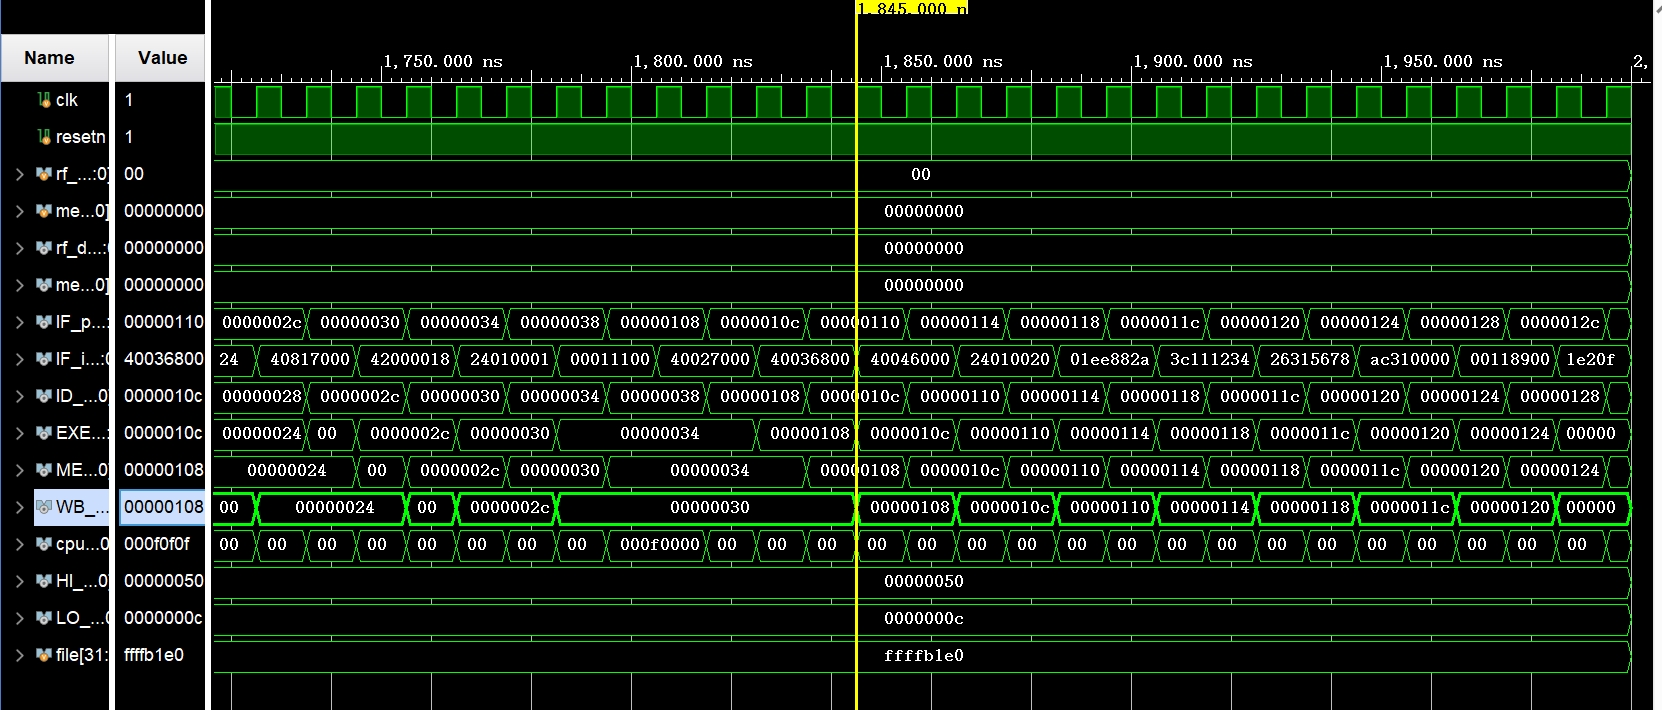
\includegraphics[width=\textwidth]{fix.png}
		\label{fig:fix}
	\end{figure}
	
	我的舍友向董前琨老师咨询了相关问题，他带回来了新的方案：直接将mfc0处理阶段前移。我当前的解决方案很明显是让mfc0踢出旁路设计回归严格阻塞，那么这部分其实就没有被优化；既然exe和mem流水级只是输出占位零值，为什么不直接将mfc0的真正所在流水级提前呢，既解决了问题，也优化了效率。
	
	
	\section{总结感想}
	通过本次实验，让我具体的理解了旁路前递设计的原理。
	
	旁路前递让五级流水 CPU 真正释放出性能潜力。通过让执行级、访存级、写回级在计算完成的第一时间把结果“递”回译码级，同时精准地控制哪些指令可以提前使用结果、哪些必须等待，我们既保留了 load、乘法、CP0 访问等指令固有的延迟，又最大限度地减少了数据依赖造成的停顿。相信后续只要能弄清楚一条指令在哪一拍产出数据、如何确认它稳定，我就能快速判断是否需要为它定制旁路策略。
	
	除此之外，通过在流水级之间添加旁路的设计过程，也加深了我对于流水线设计、各级流水级的结构功能以及相互关系的理解。
	
	还有对于mfc0出现问题的解决，也提醒了我：要真正了解每条指令的执行过程和处理逻辑设计。
	
\end{document}